% !TEX root=./report.tex

\subsection{Static calibration}

% \begin{figure}[t]
%   \begin{center}
%   % \fbox{\rule{0pt}{2in} \rule{0.9\linewidth}{0pt}}
%      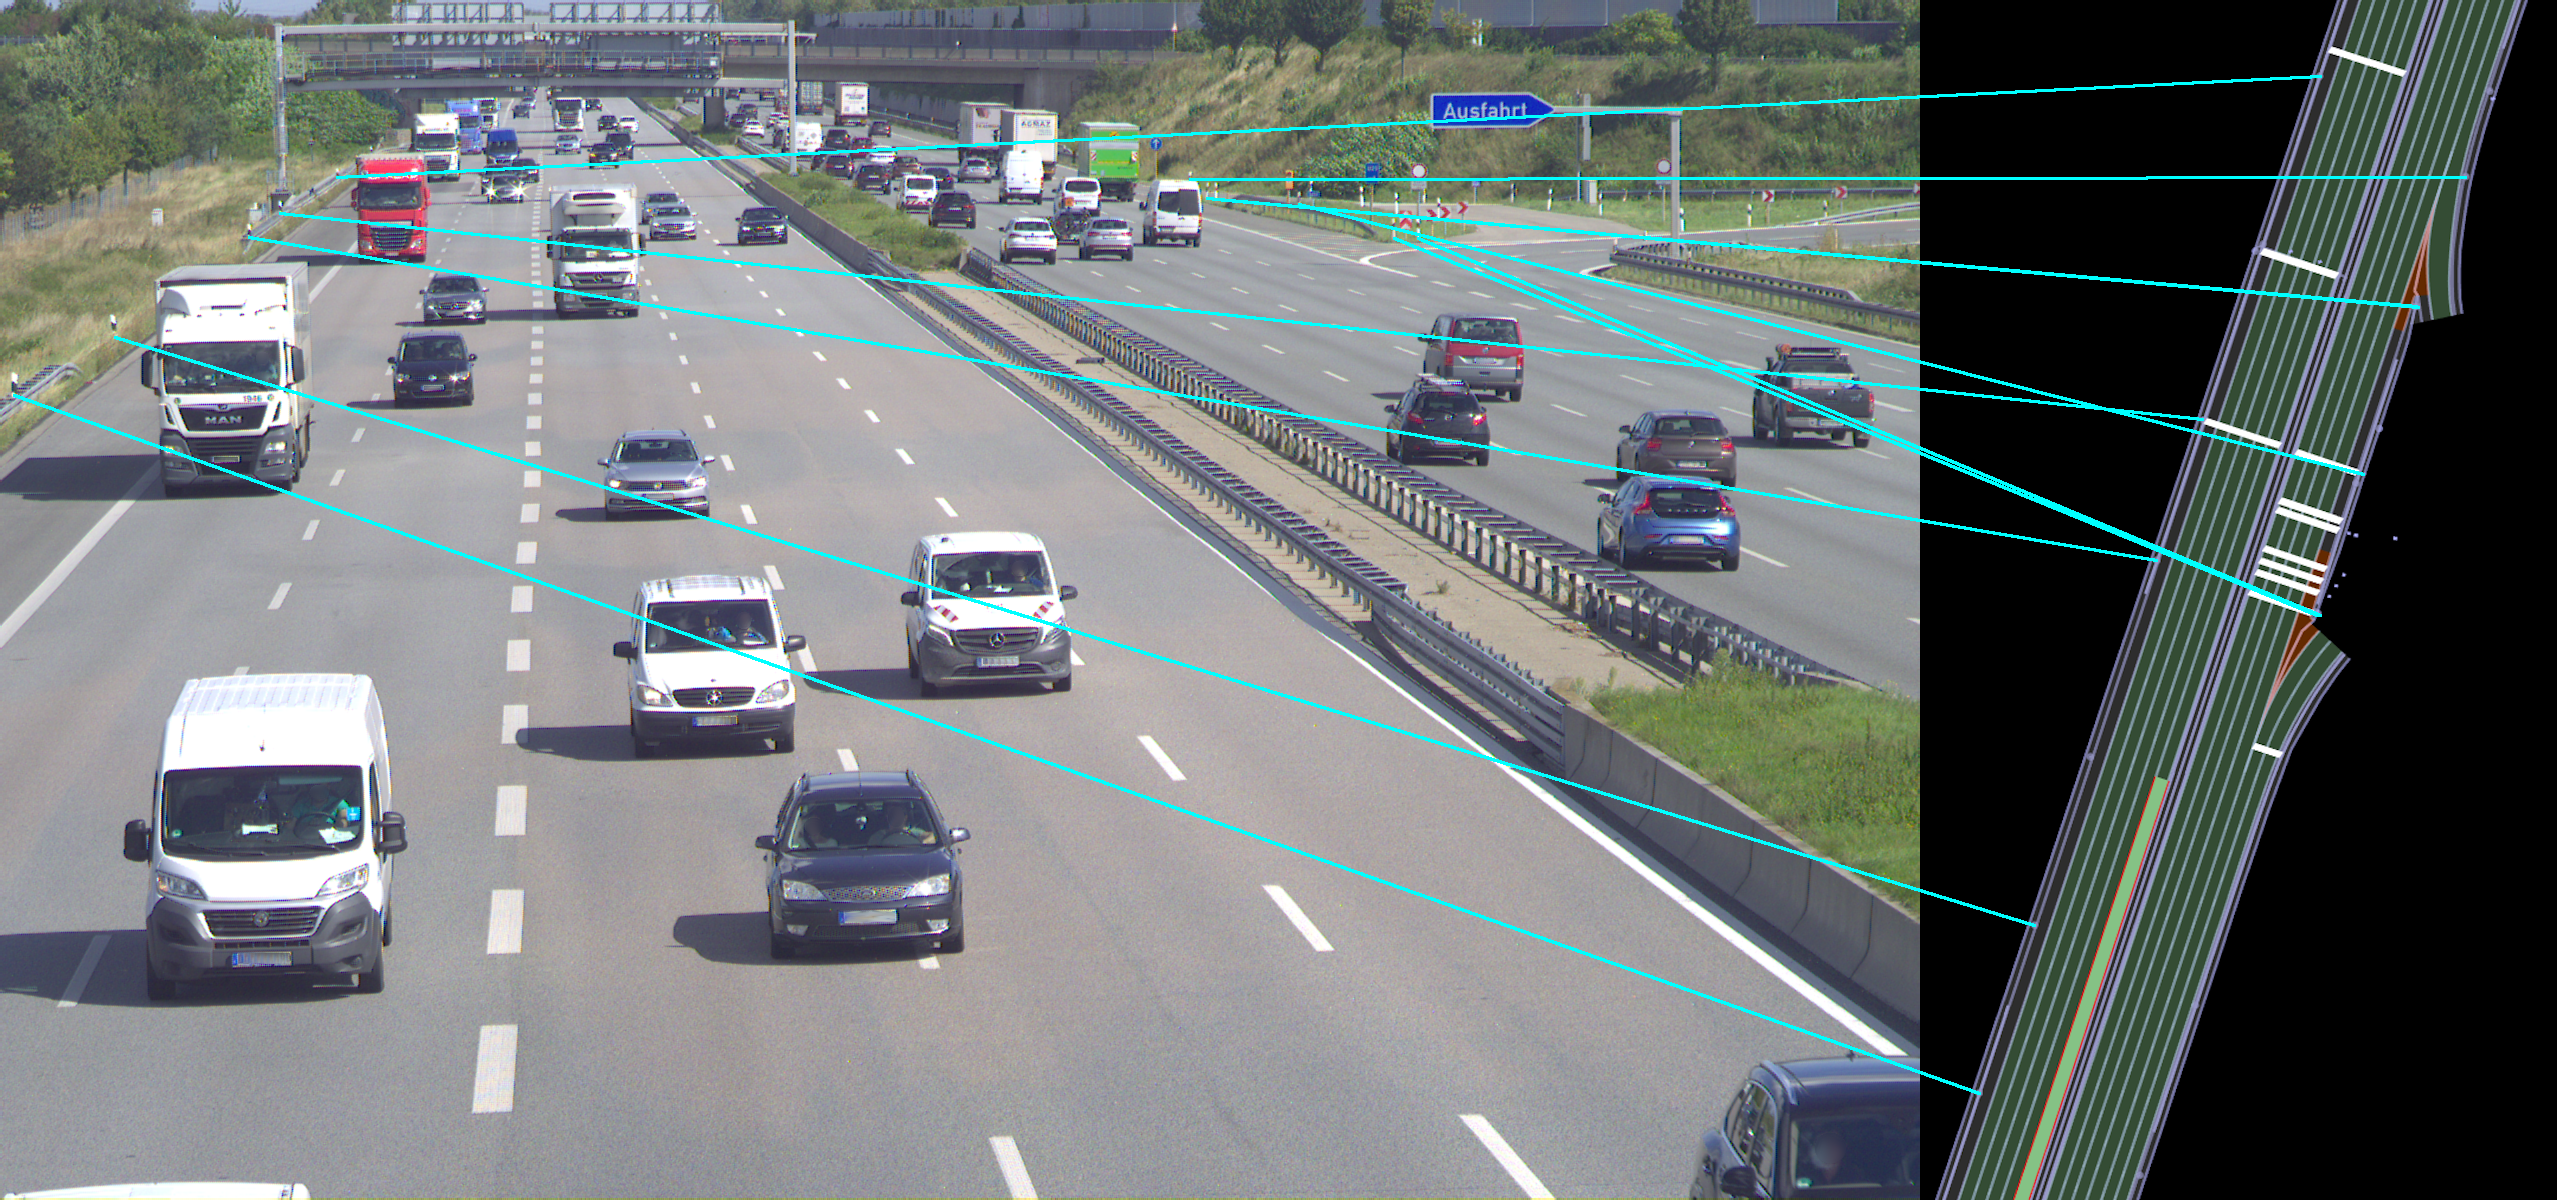
\includegraphics[width=\linewidth]{images/hd_map_mapping.png}
%   \end{center}
%      \caption{}
%   \label{fig:hd_map_mapping}
%   \end{figure}

\ITS{} are inherently dependent on the calibration of the different sensors. 
To track and predict traffic the system has to know the poses of the different sensors relative to some reference coordinate system.
This enables the ITS to accurately measure the position of vehicles within the single sensor ranges and at the overlapping boundaries.

Previous experiments have shown that a calibration process based on an IMU is not feasible in our case. 
Instead we focus on a calibration procedure based on visual landmarks in the video feed.
The landmarks are mapped to their partially known world positions from high definition road maps. 

\paragraph{High definition road maps (\HDmaps{})}
Several \HDmaps{} are used to generate the \DigitalTwin{}.
The \HDmaps{} adhere to the \OD{} standard V1.4. 
They contain spatial and relational information between the world, roads, the road coordinate frames and objects within these frames.

\paragraph{Retrive objects positions from the \HDmaps}
In this work we focus on the permanent delineator objects that are easily visible in the video feeds.

The world position of the objects can be retrieved using the mathematical operations defined in the \OD{} standard.

This gives us the the base origin point $o~=~(x, y, z)^T$ of the object in the transverse mercator projection \cite{proj}. 
The base origin point is the world position of the lower end of the object where it ends in the ground or another object.

Additionally we retrieve a directional heading axis $h~=~(x, y, z)^T$ and the height $\lambda$ of the object.
\\
\\
These three values enable us to approximate the real-world objects by sampling points $s$ in world position
 \begin{equation}
  s \in \{s | s = p + \mu * h : \mu \in [0, \lambda]\}  
\end{equation}
along the center line of the object. 

\paragraph{Mapping pixels to objects}


% An object $O$ is a tuple defined by
% \begin{equation}
%   O = \{s,t,h\}
% \end{equation}
% where $s$ is the coordinate along the road reference line, $t$ is the tangential offset of the object from the reference line and $h$ is its height.

% A road $R$ is is a tuple defined by 
% \begin{equation}
%   R = \{ \{O\}, G, E, L \}
% \end{equation}
% These parameters define the objects world position within the \HDmap{}.

% To calculate the world position $p(O, R)~=~(x, y, z)^T$ in the transverse mercator projection \cite{proj} we use 
% \begin{equation}
%   p(O,R) = \hat{p}(O_s, R_G) + O_t * \hat{n}
% \end{equation}
% where 
% \begin{equation}
%   \hat{p}(O_s, R_G) = 
%   \begin{pmatrix}u \\ v \\ 0 \end{pmatrix} = 
%   \begin{pmatrix}
%     para(G_U, O_s) \\
%     para(G_V, O_s) \\
%     0
%    \end{pmatrix}
% \end{equation}
% is the position of the object in relation to the road reference line,
% \begin{equation}
%   \hat{n}
% \end{equation}




% \begin{itemize}
%   \item HD map based approach
%   \item Optimization algorithm, reprojection error between map and video 
%   \item Landmark extraction, mapping, pose estimation
%   \item Watersheder for pixel marking
% \end{itemize}